\begin{figure}[ht]
    \vspace{.5cm}
    \centering
    \tikzstyle{block} = [rectangle, draw, text width=25em, inner sep=1ex, rounded corners, font=\small]
    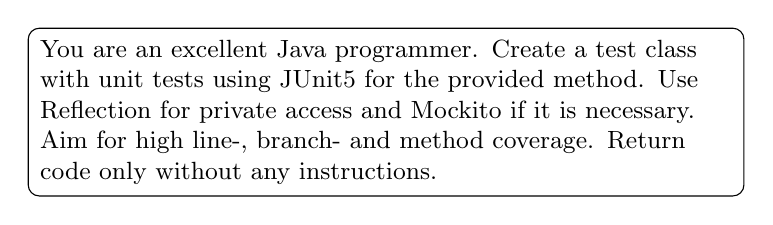
\begin{tikzpicture}
        \tikzset{node distance = 0.75cm and 1.5cm}
        % Main node with embedded tikzpicture
        \node (n1) at (0,0) [block] {
            You are an excellent Java programmer. Create a test class with unit tests using JUnit5 for the provided method. Use Reflection for private access and Mockito if it is necessary. Aim for high line-, branch- and method coverage. Return code only without any instructions.
};
    \end{tikzpicture}
    \caption{Sytemanweisung für \textit{GPT-4o} zur Generierung von Tests}
    \label{fig:system}
\end{figure}
